\documentclass[tikz,border=5pt]{standalone}
\usepackage{amsmath}
\usepackage{graphicx}
\usetikzlibrary{arrows.meta,positioning,calc}

\definecolor{arrowgray}{HTML}{333333}
\definecolor{inputfill}{HTML}{EAF1F8}
\definecolor{inputborder}{HTML}{4A6B8A}
\definecolor{baselinefill}{HTML}{FBEBD9}
\definecolor{baselineborder}{HTML}{B8702E}
\definecolor{residualfill}{HTML}{E4F2E7}
\definecolor{residualborder}{HTML}{3C7A4A}
\definecolor{correctionfill}{HTML}{EDE4F5}
\definecolor{correctionborder}{HTML}{6A4C93}
\definecolor{predictionfill}{HTML}{E3EEF9}
\definecolor{predictionborder}{HTML}{2F5F8A}
\definecolor{evaluationfill}{HTML}{F2F2F2}
\definecolor{evaluationborder}{HTML}{7F7F7F}

\begin{document}
\resizebox{8.6cm}{!}{%
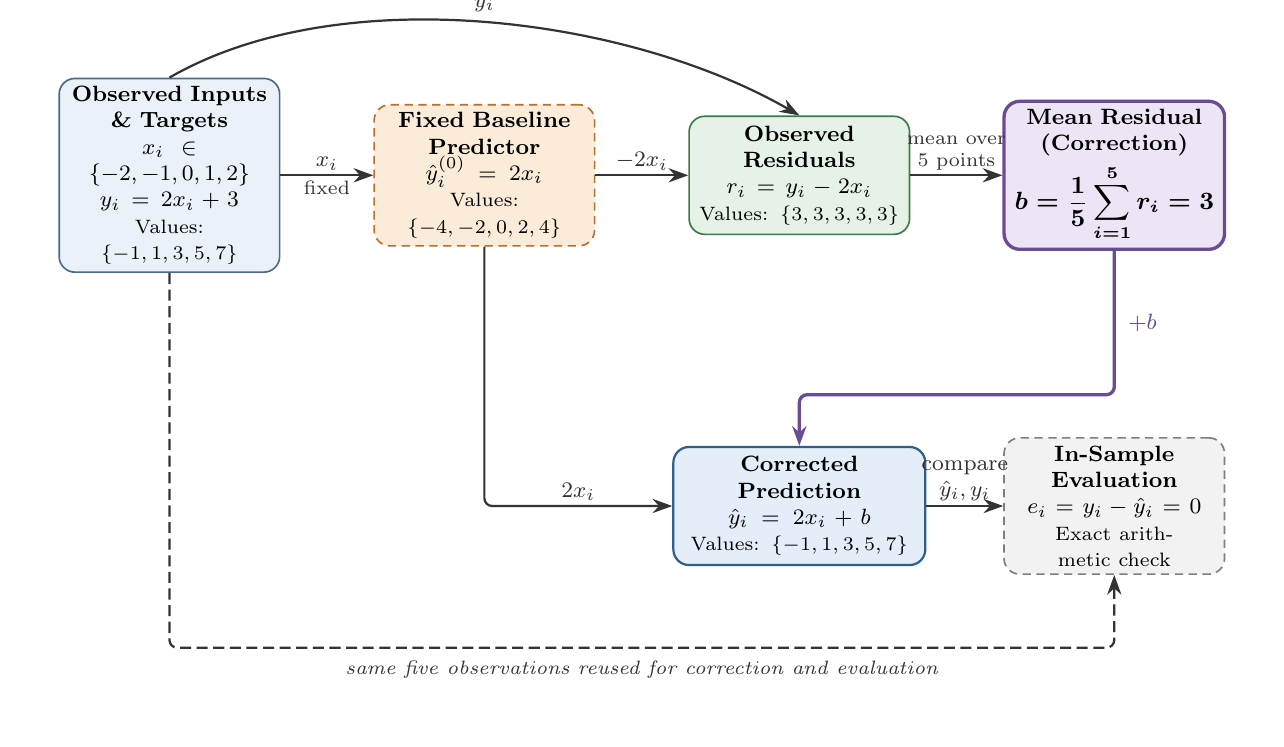
\begin{tikzpicture}[
    x=1cm,
    y=1.5cm,
    font=\normalfont,
    box/.style={
        rectangle,
        rounded corners=2mm,
        line width=0.6pt,
        minimum width=2.8cm,
        minimum height=1.5cm,
        text width=2.6cm,
        inner xsep=1mm,
        inner ysep=1mm,
        align=center,
        font=\footnotesize
    },
    flow/.style={
        -{Stealth[length=2.5mm,width=1.8mm]},
        line width=0.8pt,
        draw=arrowgray,
        rounded corners=1mm
    },
    correctionflow/.style={
        flow,
        draw=correctionborder,
        line width=1.2pt
    },
    label/.style={
        font=\footnotesize,
        text=arrowgray,
        inner sep=1.5pt,
        align=center
    }
]

% White, borderless 16:9 canvas.
\path[fill=white]
    (0,0) rectangle (15.6,5.85);
\useasboundingbox (0,0) rectangle (15.6,5.85);

\node[box,fill=inputfill,draw=inputborder]
    (inputs) at (1.8,4.6) {%
        \textbf{Observed Inputs \& Targets}\\
        $x_i\in\{-2,-1,0,1,2\}$\\
        $y_i=2x_i+3$\\
        {\scriptsize Values: $\{-1,1,3,5,7\}$}
    };

\node[box,fill=baselinefill,draw=baselineborder,
      dash pattern=on 3pt off 2pt]
    (baseline) at (5.8,4.6) {%
        \textbf{Fixed Baseline Predictor}\\
        $\hat{y}^{(0)}_i=2x_i$\\
        {\scriptsize Values: $\{-4,-2,0,2,4\}$}
    };

\node[box,fill=residualfill,draw=residualborder]
    (residuals) at (9.8,4.6) {%
        \textbf{Observed Residuals}\\
        $r_i=y_i-2x_i$\\
        {\scriptsize Values: $\{3,3,3,3,3\}$}
    };

\node[box,fill=correctionfill,draw=correctionborder,
      line width=1.2pt]
    (correction) at (13.8,4.6) {%
        \textbf{Mean Residual (Correction)}\\[2pt]
        {\small $\displaystyle
        \boldsymbol{b=\frac{1}{5}\sum_{i=1}^{5}r_i=3}$}
    };

\node[box,minimum width=3.2cm,text width=3cm,
      fill=predictionfill,draw=predictionborder,line width=0.8pt]
    (prediction) at (9.8,1.8) {%
        \textbf{Corrected Prediction}\\
        $\hat{y}_i=2x_i+b$\\
        {\scriptsize Values: $\{-1,1,3,5,7\}$}
    };

\node[box,fill=evaluationfill,draw=evaluationborder,
      dash pattern=on 3pt off 2pt]
    (evaluation) at (13.8,1.8) {%
        \textbf{In-Sample Evaluation}\\
        $e_i=y_i-\hat{y}_i=0$\\
        {\scriptsize Exact arithmetic check}
    };

\draw[flow]
    (inputs.east) --
    node[label,above] {$x_i$}
    node[label,below,font=\scriptsize] {fixed}
    (baseline.west);

\draw[flow]
    (inputs.north)
    to[out=30,in=150,looseness=0.8]
    node[label,above=2pt] {$y_i$}
    (residuals.north);

\draw[flow]
    (baseline.east) --
    node[label,above] {$-2x_i$}
    (residuals.west);

\draw[flow]
    (residuals.east) --
    node[label,above,font=\scriptsize] {mean over\\5 points}
    (correction.west);

\draw[flow]
    (baseline.south) --
    (baseline.south |- prediction.west) --
    node[label,above] {$2x_i$}
    (prediction.west);

\coordinate (correctionturn) at
    (correction.south |- {$(prediction.north)+(0,0.65cm)$});

\draw[correctionflow]
    (correction.south) --
    node[label,right=3pt,text=correctionborder]
        {\textbf{$+b$}}
    (correctionturn) --
    ($(prediction.north)+(6mm,0.65cm)$)
    -| (prediction.north);

\draw[flow]
    (prediction.east) --
    node[label,above] {compare\\$\hat{y}_i,y_i$}
    (evaluation.west);

\draw[flow,dash pattern=on 4pt off 2pt]
    (inputs.south) --
    (1.8,0.6) --
    node[label,below=3pt,font=\scriptsize\itshape]
        {same five observations reused for correction and evaluation}
    (13.8,0.6) --
    (evaluation.south);

\end{tikzpicture}%
}
\end{document}